\documentclass[12pt]{article}
\usepackage{authblk}
\usepackage[margin=1in]{geometry}
\geometry{letterpaper}
\usepackage{graphicx}
\usepackage{amssymb}
\usepackage{amsmath}

\usepackage[style=nature, natbib=true, autocite = superscript]{biblatex}
\addbibresource{../superStat.bib}
\let\citep=\autocite

\usepackage{lineno}
\usepackage{paralist}

%% for citing stuff in the supp
\usepackage{xr}
\externaldocument{rom_natComm_supp}


\title{Punctuated non-equilibrium and niche conservatism explain
biodiversity fluctuations through the Phanerozoic}

\author[1]{Andrew J. Rominger} 
\author[2, 3, 4]{Miguel A. Fuentes}
\author[2, 5, 6, 7, 8]{Pablo A. Marquet}

\affil[1]{Department of Environmental Science, Policy and Management,
University of California, Berkeley}
%
\affil[2]{Santa Fe Institute, 1399 Hyde Park Road, Santa Fe, New
Mexico 87501, US}
%
\affil[3]{Instituto de Investigaciones Filos\'oficas, SADAF, CONICET,
Bulnes 642, 1428 Buenos Aires, Argentin}
%
\affil[4]{Facultad de Ingenier\'ia y Tecnolog\'ia, Universidad San
Sebasti\'an, Lota 2465, Santiago 7510157, Chile}
%
\affil[5]{Departamento de Ecolog\'ia, Facultad de Ciencias
Biol\'ogicas, Pontificia Universidad de Chile, Alameda 340, Santiago,
Chile}
%
\affil[6]{Instituto de Ecolog\'ia y Biodiversidad, Casilla 653,
Santiago, Chile}
%
\affil[7]{Laboratorio Internacional de Cambio Global (LINCGlobal),
Pontificia Universidad Católica de Chile, Alameda 340, Santiago,
Chile}
%
\affil[8]{Centro Cambio Global UC, Av.~Vicu\~na Mackenna 4860, Campus
San Vicu\~na, Santiago, Chile}

\date{}

\begin{document}

\maketitle

\clearpage
\linenumbers

\begin{abstract}
Fluctuations in biodiversity, both large and small, are pervasive
through the fossil record, yet we do not understand the processes
generating them.
% 
Here we use a novel extension of theory from non-equilibrium
statistical physics to show that three universal properties of
macroevolution, punctuated adaptive radiation, niche conservatism and
resultant heterogeneity of diversification rates between taxa, are
sufficient to explain previously unaccounted for biodiversity patterns
throughout the Phanerozoic.
% 
Using this theory, known as super-statistics, we identify taxonomic
orders as largely autonomous evolutionary units, each likely
experiencing its own unique and conserved adaptive landscape.  This
indicates that while neutral processes could adequately explain
within-order diversification, between-order diversification is likely
driven by major evolutionary innovations.
% 
Super-statistics, has been successfully used to explain other
complex systems including driven turbulent flows and wild stock market
fluctuations.
% 
Compared to other approaches that have used simple birth-death
processes, equilibrial dynamics or non-linear theories from complexity
science, super-statistics is superior in its ability to account for
both small and extreme fluctuations in fossil diversity.
% 
Its success opens up new research directions to better understand
the evolutionary processes leading adaptive landscapes to be conserved
within orders and undergo punctuated innovations between orders.
\end{abstract}

\clearpage

%% Diversity changes
Biodiversity has not remained constant nor followed a simple
trajectory through geologic time \citep{raup1982, sepkoski1984,
  gilinsky1994, liow2007, alroy08, alroy2010}.  Instead, it has been
marked by fluctuations in the number of extant taxa, both positive in
the case of net origination or negative in the case of net
extinction. Major events, such as adaptive radiations and mass
extinctions have received special attention \citep{benton1995,
  Erwin1998}, but fluctuations of all sizes are ubiquitous
\citep{sepkoski1984, alroy08, quental2013}. Predicting the magnitude
of these fluctuations continues to illude paleobiologists and
biodiversity theoriticians.

%% What drives diversity dynamics?
Several approaches have been taken to study the complex trajectory of
paleo-biodiversity ranging from the hypothesis that biological systems
self-organize to the brink of critical phase-transitions
\citep{bak1993, sole1997} to invocations of non-linear environmental
perturbations \citep{newman1995} and escalatory co-evolutionary
interactions \citep{vermeij1987}. New data and analyses have not
supported any of these hypotheses at the scale of the entire
Phanerozoic marine invertebrate fauna \citep{kirchner1998, madin2006,
  alroy08}. Other studies have modeled the mean trend in diversity as
tracking a potentially evolving equilibrium \citep{sepkoski1984,
  alroy08, alroy2010, rabosky2009ecolLett} and yet ignore the
potential role of stochasticity and non-equilibrium dynamics in
producing observed patterns \citep{erwin2012, liow2007,
  quental2013}. As such, we still lack a synthetic theory of evolving
biodiversity through the fossil record.
%
Here we build a parsimonious theory of diversification across an
adaptive landscape, deriving predictions from universal
non-equilibrial processes, and show that it accurately predicts the
complex distribution of pervasive diversity fluctuations throughout
the marine Phanerozoic.

\subsection*{Diversification in an Adaptive Landscape}

Model: takes from classic models (simpson, wright) says
diversification in a region of niche space is equilibrial. Constraints
on evolutionary innovation (i.e. niche conservatism) lead to stasis in
those niches. Underlying properties of that region of niche space
determine rates of orig and extinct leading to different
$\beta$. Result is different Gaussians in different regions and a jump
process between regions (e.g. Gamma).

This is same as super-stats. Stat mech in biodiversity has powerful
potential.

Predictions

Datasets

Despite the heterogeneity of explanations of Phanerozoic
biodiversity, consensus has emerged on three properties of
macroevolution:
\begin{inparaenum}[\itshape i\upshape)]
\item gross ecological and life history attributes of clades
  (i.e. groups of related species descending from a common ancestor)
  are often maintained, a phenomenon known as niche conservatism
  \citep{roy2009range, hopkins2014};
\item long periods of niche conservatism are interrupted by adaptive
  diversification and exploration of new ecological niche space
  \citep{eldredgeGould1972, newman1985adaptive, hopkins2014}; and
\item as a consequence of the interaction between their life history
  characteristics and the dynamics of the environments they inhabit
  \citep{vrba1983} different clades experience different rates of
  morphological evolution, speciation and extinction
  \citep{simpson1953, sepkoski1984, holman1989, gilinsky1994}.
\end{inparaenum}

%% bring up punctuated equilib is actually non-equilibrium and explain
%% title
Observed bursts of adaptive radiation leading to novel morphologies in
the fossil record led Eldredge and Gould to their hypothesis of
punctuated equilibrium \citep{eldredgeGould1972}. Here we show that
this punctuation is actually akin to the ``super statistical theory''
of non-equilibrium dynamics in statistical physics
\citep{beck2003}. Super-statistics \citep{beck2003} proposes that
non-equilibrial systems can be decomposed into locally equilibrial
sub-systems. The distribution of equilibria across sub-systems
determines the dynamics of the complete system \citep{beck2003}. When
these sub-systems are superimposed the resulting system can no longer
be described by a single equilibrial model. In the context of
macroevolution we propose that a clade with conserved life history
characteristics corresponds to a locally equilibrial sub-system. If a
certain region of niche space can only contain a finite diversity of
taxa \citep{simpson1953, gavrilets2005, rabosky2009ecolLett, price2014}
then diversity within clades should fluctuate stochastically about
this equilibrium due to random origination and extinction. The
magnitude of these macroevolutionary rates should be a function of the
life history and ecological characteristics that define that region of
niche space. Larval type \citep{jablonski2008}, body plan
\citep{erwin2012}, body size \citep{harnik2011}, range size
\citep{harnik2011, foote2008paleobiol} and substrate preference
\citep{hopkins2014} have all been shown to influence such rates. Thus
different regions of niche space, and the clades occupying them, will
experience different magnitudes of stochastic fluctuation in
diversity. As clades occasionally split to fill new regions of niche
space their punctuated diversification determines the non-equilibrium
nature of the entire biota. Here we show that these properties of
macroevolution are sufficient to explain the complex fluctuations of
marine invertebrate diversity through the Phanerozoic.

%% connect idea of a 'statistic' to evol
In statistical mechanics, local sub-systems can be defined by a simple
statistical parameter $\beta$ often corresponding to inverse
temperature. In the context of macroevolution we define $\beta$ as the
inverse variance of a homogenous origination-extinction process, which
will capture all relevant information about a clade's diversification
under such a process.  The limit distribution of time averaged
fluctuations in clade $k$'s diversity through time should be
approximately Gaussian with variance $1/\beta_k$ (Appendix
\ref{sec:suppLimitDist}). We posit that just as in statistical
systems, non-equilibrium dynamics can arise from the mixing of the
dynamics of many locally equilibrial subsystems. For marine
Phanerozoic diversity this corresponds to mixing the dynamics of many
clades, all being described by their unique $\beta_k$ values.  Three
exemplar dynamics taken from a bias-corrected (see methods section)
aggregation of the Paleobiology Database (PBDB) \citep{alroy08} are
shown in Figure \ref{fig:pk_f}.
%% should talk about alternatives to neutrality?  i.e. bd process but
%% enviro could drive it too (cite Peters) but neutral drift is sufficient.
To predict the super-statistical behavior of the entire marine
invertebrate Phanerozoic fauna we must integrate over all possible
local equilibria that each clade could experience. The distribution of
$\beta_k$ values describes the probability that a given clade, chosen
at random, will occupy a region of niche space characterized by that
inverse variance value. The form of this stationary distribution of
$\beta_k$ values could shed interesting light on the biological
processes that lead different clades to different equilibria, as
discussed below.  Figure \ref{fig:pk_f} shows the shape of this
stationary distribution estimated from bias-corrected PBDB
\citep{alroy08} data.

%% now talk about actual data and results
% to test our model we do all this: methods interlude
To uncover the super-statistical nature of the marine invertebrate
Phanerozoic fauna we analyze the distribution of diversity
fluctuations using two canonical databased of fossil biodiversity, the
PBDB \citep{alroy08} and Sepkoski's compendium \citep{sepkoski1992} of
fossil marine invertebrates (results from Sepkoski's compendium are
presented in Appendix \ref{sec:suppSepk}).  We filter PBDB
data to include only well preserved marine invertebrates following
previously published collection inclusion criteria \citep{alroy08,
  alroy2010}.  We account for detection bias in the PBDB using an
extension of the ``three timer'' correction \citep{alroy08}. ``Three
timer'' correction accounts for the rate of failure to observe a
genus, estimated by the number of times a gap occurs in its occurrence
history. We extend this correction by also employing a new publication
bias correction to help eliminate bias from preferential publication
of novel taxa (see methods section). Results obtained from this
correction strategy are similar to other published methods
(Fig. \ref{fig:supp_3TPub}). Fluctuations within a clade are computed
as the difference in standing diversity between two time intervals, or
equivalently the number of originations minus extinctions in one
interval.

%% Different potential ways of breaking up taxa into clades
Phanerozoic biodiversity can be deconstructed and grouped into clades,
or sub-systems, in several different ways. Lacking a full phylogenetic
hypothesis for all marine invertebrates we use taxonomic
classifications to identify potential sub-systems.  Taxa ideally
represent groups of organisms that descend from a common ancestor and
share similar ecologically and evolutionary relevant morphological
traits \citep{mayr1965systZool, erwin2007}.  For Phanerozoic marine
invertebrates, Holman \citep{holman1989} has shown that variance in
diversity dynamics is less between taxa belonging to the same order
than taxa in different orders, indicating that the taxonomic level of
orders is a likely candidate for sub-system delineation. To evaluate
the optimal taxonomic level for sub-system designation, we test our
superstatistical theory using taxonomic levels from order through
class to phylum. Additionally we compare our results to randomized
taxonomies to confirm that observed patterns are not an artifact of
arbitrary classification but instead represent real biologically
relevant differences between clades.



\section{Results and Discussion}
% present p_k(x|b), f(b) and P(x) fit
At the order level in both the sampling-corrected PBDB
(Fig. \ref{fig:pk_f}) and Sepkoski's compendium (Appendix
\ref{sec:suppSepk}), fluctuations in genus diversity are well
described by a Gaussian distribution (Fig. \ref{fig:pk_f}). Gaussian
fluctuations would result from a homogeneous origination-extinction
process under the condition of independence between
orders. Independence could result from neutral-like processes
\citep{hubbell2001}, where the dynamics of one taxon are unaffected by
those of another, or from dampening mechanisms that stabilize complex
networks of interacting taxa \citep{brose2005}. This is in direct
contrast to the instability hypothesis underlying the self-organized
criticality theory of paleo-biodiversity \citep{bak1993, sole1997}.

We estimate the distribution of $\beta_k$'s simply as the maximum
likelihood distribution describing the set of inverse variances for
all orders. In both the PBDB and Sepkoski's compendium, Phanerozoic
marine invertebrate orders clearly follow a Gamma distribution in
their $\beta_k$ values (Fig. \ref{fig:pk_f}).  While multiple
processes could lead to a Gamma stationary distribution
\citep[e.g.][]{cir1985}, one interesting possibility is a
mean-reversion process \citep{cir1985}. Mean reversion could be a
consequence of niche conservatism if $\beta_k$ values are associated
with a clade's physiological and life history traits, themselves
evolving via Ornstein-Uhlenbeck-like exploration of an adaptive
landscape \citep{cir1985, butler2004}.

Using the observation of within order statistical equilibrium and
Gamma-distributed $\beta_k$ parameters we can calculate, without
further adjusting free parameters, the distributions of order-level
fluctuations for the entire marine Phanerozoic, $P(x)$, as
\begin{equation}
  P(x) = \int_0^\infty p_k(x \mid \beta) f(\beta) d\beta \label{eq:PxInt}
\end{equation}
where $p_k(x \mid \beta)$ is the distribution of fluctuations within
an order and $f(\beta)$ is the stationary distribution of inverse
variance in the magnitude of order-level fluctuations in
diversity. This leads to a non-Gaussian, fat-tailed prediction for
$P(x)$ which matches both the PBDB and Sepkoski data closely
(Fig. \ref{fig:Px} and Appendix \ref{sec:suppSepk}).

To quantitatively evaluate how well the super-statistical prediction
matches the data we constructed a 95\% confidence envelope from
bootstrapped maximum likelihood estimates for $P(x)$. Observed
fluctuations fall within this 95\% confidence envelope
(Fig. \ref{fig:Px}), indicating that the data do not reject the
super-statistical prediction. For further comparison, we fit a
Gaussian distribution to the observed fluctuations, which corresponds
to the equilibrium hypothesis that all orders conform to the same
statistics. Using Akaike Information Criterion (AIC) we find that
observed fluctuations are considerably better explained by the
super-statistical prediction than by the Gaussian hypothesis ({\small
  $\Delta$}AIC = 11285.18). Thus, as expected under the
super-statitical hypothesis, the fat tailed distribution of
fluctuations arise from the superposition of independent Gaussian
statistics of fluctuations within orders.

%% calculating sstat at different taxonomic levels (D-stat fig)
Computing the distribution of fluctuations using classes instead of
orders leads to a substantially poorer fit to the observed data
(Fig. \ref{fig:supp_PBDB_Px_cls}). We quantify this shift with the
Kolmogorov-Smirnov statistic, which changes from 0.041 for orders to
0.062 for classes (Fig. \ref{fig:dStat}). However, if super-statistical
theory explains the data, this worsening fit with increasing taxonomic
scale is expected as the different classes are not well defined
subsystems in their fluctuation dynamics. Instead, classes aggregate
increasingly disparate groups of organisms, and thus effectively mix
their associated Gaussian fluctuations, meaning that one statistic
should no longer be sufficient to describe class-level dynamics. Our
analysis indicates that orders are evolutionarily coherent and
independent entities, with all subsumed taxa sharing key ecological
and evolutionary attributes allowing them to diversify concertedly and
independently from other orders. Both the good fit at the order level
and worsening fit at higher taxonomic levels is confirmed in
Sepkoski's compendium, which also allows analysis of phylum-level
patterns (Fig. \ref{fig:supp_sepkPx}).

To further test the evolutionary coherence of orders we conducted a
permutation experiment in which genera were randomly reassigned to
orders while maintaining the number of genera in each order. For each
permutation, we calculated the super-statistical prediction and the
Kolmogorov-Smirnov statistic. The permutation simulates a null model
in which common evolutionary history is stripped away (genera are
placed in random orders) but the total number of observed genera per
order is held constant.  Repeating this permutation 500 times yields a
null distribution of Kolmogorov-Smirnov statistics that is far
separated from the observed value (Fig. \ref{fig:dStat}) suggesting
the good fit at the order level is not merely a statistical artifact
of classification but carries important biological information.

\section{Conclusions}

%% why orders
Our analysis makes no assumption that orders should correspond to
super-statistical subsystems, but identifies them as the appropriate
level for marine invertebrates. Holman \citep{holman1989} has also
shown that orders are ``evolutionarily coherent'' in that subtaxa
within orders share common diversification dynamics. As we show,
orders differ only in the variances of their diversity fluctuations
(Fig. \ref{fig:pk_f}).

Our study is the first to demonstrate that complex patterns in the
sequence of origination and extinction events in the fossil record are
the result of a simple underlying process analogous to the statistical
mechanisms by which complexity emerges in large, non-equilibrium
physical \citep{beck2004} and social systems \citep{fuentes2009}.  We
do so by identifying the biological scale at which clades conform to
equilibrial dynamics. This scale is likely determined by the process
of niche conservatism \citep{} within orders, and equilibrium the
likely outcome of neutrality or processes that dampen---rather than
exacerbate---fluctuations in complex ecological networks \citep{}. We
then show that punctuated shifts to different equilibria between
order, a consequence of punctuated exploration of niche space by newly
evolving clades \citep{}, leads to a characteristically
non-equilibrial distribution of diversity fluctuations when the marine
Phanerozoic fauna is viewed as a whole macro-system.

%%% how this motivates future work in figuring out the details of
%%% biotic evolution that are important for driving stasis and
%%% punctuation
Our work highlights the importance of both niche conservatism and
punctuated adaptive radiation in producing the statistical behavior of
the Phanerozoic; our theory thus provides new motivation for
identifying the eco-evolutionary causes of innovations between
lineages and how those innovations are eventually conserved within
lineages. Armed with an understanding of the statistical behavior of
diversification we can go on to examine mechanisms underlying
additional patterns in the mean trend of biodiversity through the
Phanerozoic. In particular, clades have been shown to wax and wane
systematically through time \citep{liow2007,
  quental2013}, a pattern that we cannot explain with super-statistics
alone.

%% section on thinking about meaning of beta ~ Gamma cut, may have
%% been redundant see `#2'

%% note on how sstat could be applied to other questions in eco-evo.
Super-statistics could also be applied to other areas of evolution and
macroecology.  For example new phylogenetic models already consider
heterogeneous rates of diversification
\citep[e.g.][]{rabosky2006laser}. The super-statistics of clades in
adaptive landscapes could provide a means to build efficient models
that jointly predict morphological change and diversification. This
framework could also provide a new paradigm in modeling the
distributions of diversity, abundance and resource use in non-neutral
communities. Non-neutral models in ecology are criticized for their
over-parameterization \citep{rosindell2011TREE}, yet a persistent
counter argument to neutral theory \citep{hubbell2001} is the
unrealistic assumption of ecological equivalency
\citep{chave2004neutral} and poor prediction of real dynamics
\citep{ricklefs2006neutral}. If ecosystems are viewed as the
super-position of many individualistically evolving clades, each
exploiting the environment differently and thus obeying a different
set of non-equivalent statistics, then diversity dynamics could be
parsimoniously predicted while incorporating real biological
information on ecological differences between taxa.

\section{Methods}

\subsection{Paleobiology Database data download and filtering}
Data were downloaded from the Paleobiology Database (PBDB;
www.pbdb.org) on 28 May 2013. Collections were filtered using the same
approach as Alroy \citep{alroy08} to insure that only well preserved
marine invertebrate occurrences were used in subsequent analysis
resulting in 221202 genus occurrences. These were further filtered to
exclude those occurrences without order-level taxonomy and those
collections with age estimate resolutions outside the 10my default
bins of the PBDB resulting in 189516 occurrences left for analysis. To
avoid basic sampling concerns we excluded the earliest Cambrian and
the Cenozoic.

To focus attention on the variance of fluctuations we center each
clade's fluctuation distribution. Because ``equilibrium'' in the
statistical mechanical sense means a system undergoes coherent,
concerted responses to perturbation the mean trend line is of less
interest than deviations from it. We also note that most clades are
already close to centered and so centering has little influence on
clade-specific fluctuation distributions.

\subsection{Three-timer and publication bias correction} 
\label{sec:3TP}
We use a new and flexible method, described below, to correct for
known sampling biases in publication-based specimen databases
\citep{alroy08, alroy2010}.  We were motivated to use this method
because rarefaction has been shown to under-perform compared to the
more data-intensive shareholder quorum subsampling (SQS) method
\citep{alroy2010}.  However, subsampling cannot be applied to small
orders (i.e. the majority) because SQS becomes increasingly unreliable
as sample size decreases \citep{alroy2010}.  We therefore develop a
simple method based on first correcting for detection bias using the
``three timer'' correction \citep{alroy08} in which the rate of failure
to observe a genus is estimated by the number of times a gap occurs in
the occurrence history of each genus. To eliminate further bias due to
preferential publication of novel taxa we divide observed number of
genera per order per time period by the expected number of genera
given publications in that time period.  The expected number is
calculated by regressing the log-transformed number of genera on
log-transformed number of publications. There is a weak trend toward
higher diversity with more publications (Fig. \ref{fig:divByPub})
meaning that the most important correction comes from the three timer
correction.

Our new method effectively re-scales each genus occurrence from 0/1
(absent/present), to a weighted number continuously ranging between 0
and 1.  This method achieves similar results to more computationally
intensive sub-sampling procedures \citep{alroy08, alroy2010}. We
directly compare our predicted time series of global genus diversity
with results derived from SQS \citep{alroy2010} and the raw data
(Fig. \ref{fig:supp_3TPub}).  Our method shows minor differences with
the SQS prediction, However, these discrepancies do not have impact
the distribution of fluctuations (Fig. \ref{fig:supp_3TPub}) and
super-statistical analysis on uncorrected PBDB data (see section
\ref{sec:rawPBDB}) produces a similar result to the analysis on
corrected PBDB data presented in the main text.

\subsection{Numerical methods} \label{sec:numMeth} To fit our
super-statistical prediction we use the method of least squares
instead and maximum likelihood. When building the prediction for
$P(x)$ by calculating order-level Gaussian distributions and
integrating over them, we use least squares to fit the variance term
to each order. We do so because orders potentially show asymmetries in
their distribution of fluctuations. Least squares is more flexible in
fitting such distributions compared to maximum likelihood which will
always estimate the empirical variance as the best-fitting parameters.

We also estimate $P(x)$ directly from the raw data using maximum
likelihood to compare the fit of our super-statistical prediction and
that of a simple Gaussian distribution using AIC. To calculate a
likelihood-based confidence interval on our prediction we bootstrapped
the data, subsampling fluctuations with replacement from all orders
combined.

\section*{Acknowledgments}
We thank John Harte, Rosemary Gillespie and Jun Ying Lim for helpful
discussion. Michael Foote provided a digitized copy of Sepkoski's
compendium. AJR thanks funding sources Fulbright Chile and the
National Science Foundation Graduate Research Fellowship Program; MAF
thanks FONDECYT 1140278; PM thanks support from Grant PFB-023
(CONICYT) and ICM-P05-002.

\printbibliography

\clearpage

\section*{Figures}

\begin{figure}[!h]
  \centering
  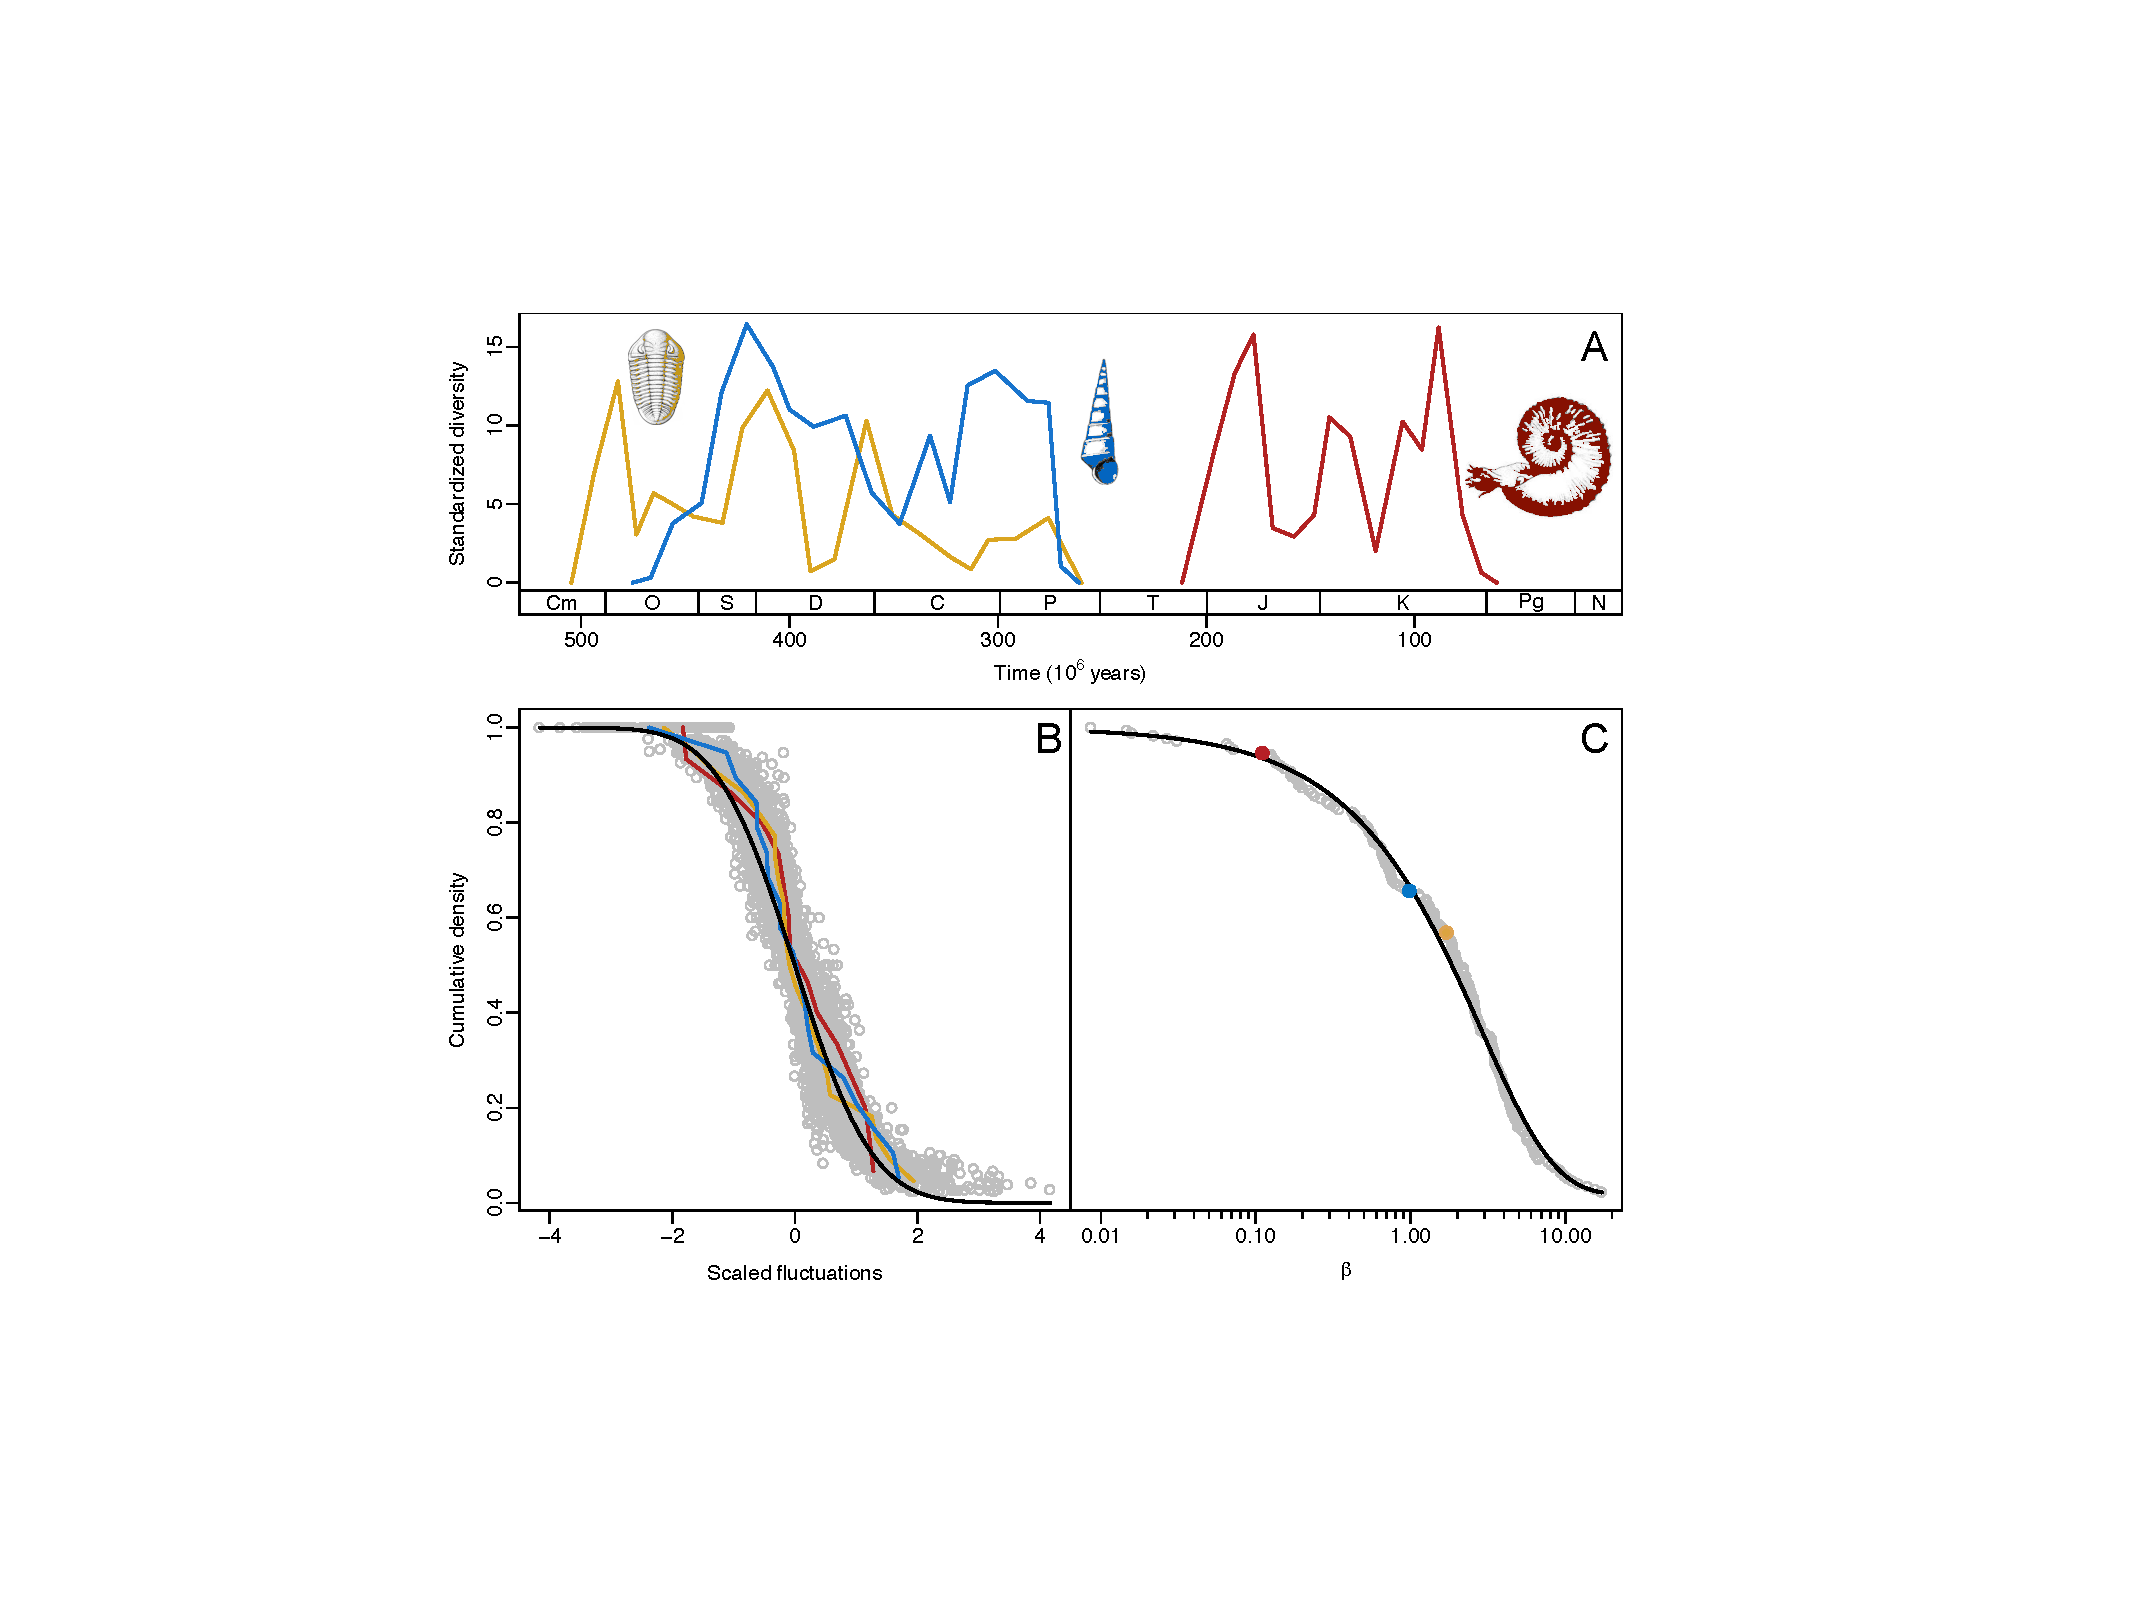
\includegraphics[scale=0.8]{figs/fig_pkx-fbeta.pdf}
  \caption[Variability in trajectories of within-order fluctuations in
  genus diversity]{The distributions of within-order fluctuations in
    genus diversity shown for the trajectories of three exemplar
    orders (A) and shown as an empirical cumulative density aggregated
    across all orders (B). To display all orders simultaneously we
    simply collapse their fluctuation distributions by dividing by
    their standard deviations. If orders conform to the Gaussian
    hypothesis their scaled fluctuations should fall along the
    cumulative density line of a normal N(0, 1) distribution, as shown
    in (B). In (C) the distribution of inverse variances $\beta_k$
    across all orders matches very closely to a Gamma distribution
    (black line); exemplar orders are again highlighted.}
  \label{fig:pk_f}
\end{figure}

\begin{figure}[!h]
  \centering
  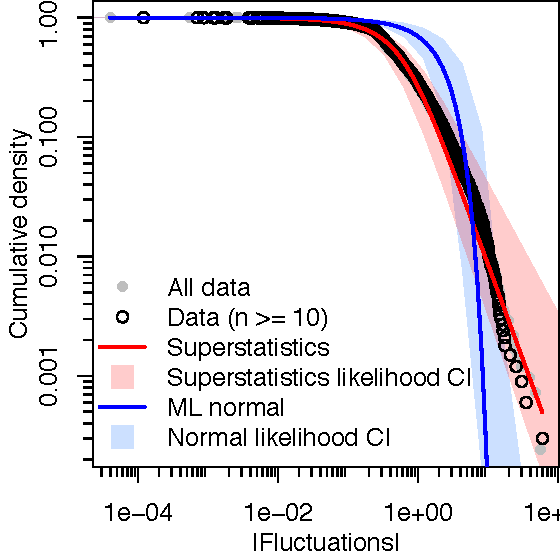
\includegraphics[scale=1]{figs/fig_Px.pdf} 
  \caption[Order-level distribuiton of diversity
  fluctuations]{Distribution of fluctuations in genus diversity within
    orders of marine invertebrates in the Paleobiology Database
    \citep{alroy08} after bias correction. The distribution is
    fat-tailed as compared to the maximum likelihood estimate of the
    normal distribution (blue line).  At the order level the empirical
    distribution of fluctuations are well described by our
    super-statistical approach, both when computed from integrating
    over the distribution of observed variances (red line) and when
    fit via maximum likelihood (95\% confidence interval; red
    shading).}
  \label{fig:Px}
\end{figure}

\begin{figure}[!h]
  \centering
  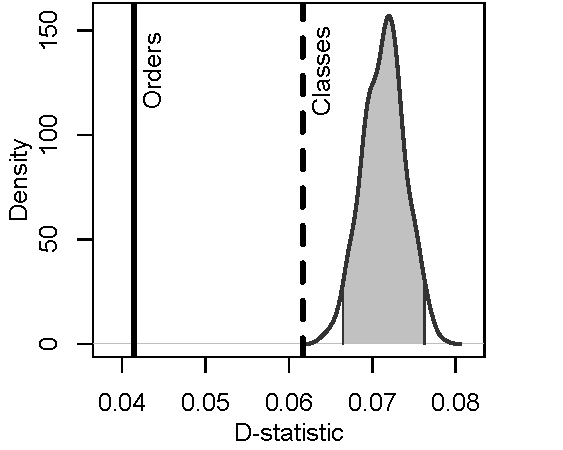
\includegraphics[scale=1]{figs/fig_dStat(3TP).pdf}
  \caption[Goodness of super-statistical theory fit]{Distribution of
    Kolmogorov-Smirnov (KS) statistics from randomly permuting genera
    within orders (gray shading represents 95\% confidence
    interval). Solid black line is observed KS statistic at the order
    level, while the dashed black line shows the observed KS statistic
    at the class level.}
  \label{fig:dStat}
\end{figure}

\end{document}